\pdfinfoomitdate=1
\pdftrailerid{}
\pdfsuppressptexinfo=15
\documentclass[11pt]{article}
\usepackage[T1]{fontenc}
\usepackage{lmodern}
\ifdefined\pdfglyphtounicode
  \ifdefined\pdfgentounicode
    \pdfgentounicode=1
  \fi
  \pdfglyphtounicode{tfm:lmex10/bracketleftbig}{005B}
  \pdfglyphtounicode{tfm:lmex10/bracketrightbig}{005D}
  \pdfglyphtounicode{tfm:lmex10/parenleftbigg}{0028}
  \pdfglyphtounicode{tfm:lmex10/parenrightbigg}{0029}
  \pdfglyphtounicode{tfm:lmex10/braceleftbigg}{007B}
  \pdfglyphtounicode{tfm:lmex10/bracerightbigg}{007D}
  \pdfglyphtounicode{tfm:lmex10/parenleftBigg}{0028}
  \pdfglyphtounicode{tfm:lmex10/parenrightBigg}{0029}
  \pdfglyphtounicode{tfm:lmex10/braceleftBigg}{007B}
  \pdfglyphtounicode{tfm:lmex10/bracerightBigg}{007D}
  \pdfglyphtounicode{tfm:lmex10/parenlefttp}{239B}
  \pdfglyphtounicode{tfm:lmex10/parenrighttp}{239E}
  \pdfglyphtounicode{tfm:lmex10/bracelefttp}{23A7}
  \pdfglyphtounicode{tfm:lmex10/braceleftbt}{23A9}
  \pdfglyphtounicode{tfm:lmex10/braceleftmid}{23A8}
  \pdfglyphtounicode{tfm:lmex10/braceex}{23AA}
  \pdfglyphtounicode{tfm:lmex10/parenleftbt}{239D}
  \pdfglyphtounicode{tfm:lmex10/parenrightbt}{23A0}
  \pdfglyphtounicode{tfm:lmex10/circleplusdisplay}{2A01}
  \pdfglyphtounicode{tfm:lmex10/summationtext}{2211}
  \pdfglyphtounicode{tfm:lmex10/uniontext}{22C3}
  \pdfglyphtounicode{tfm:lmex10/intersectiontext}{22C2}
  \pdfglyphtounicode{tfm:lmex10/summationdisplay}{2211}
  \pdfglyphtounicode{tfm:lmex10/uniondisplay}{22C3}
  \pdfglyphtounicode{tfm:lmex10/intersectiondisplay}{22C2}
  \pdfglyphtounicode{tfm:lmex10/coproductdisplay}{2210}
  \pdfglyphtounicode{tfm:lmsy10/mapsto}{23D0}
  \pdfglyphtounicode{tfm:lmsy10/B}{212C}
  \pdfglyphtounicode{tfm:lmsy10/C}{1D49E}
  \pdfglyphtounicode{tfm:lmsy10/I}{2110}
  \pdfglyphtounicode{tfm:lmsy10/J}{1D4A5}
  \pdfglyphtounicode{tfm:lmsy10/K}{1D4A6}
  \pdfglyphtounicode{tfm:lmsy10/M}{2133}
  \pdfglyphtounicode{tfm:lmsy10/T}{1D4AF}
  \pdfglyphtounicode{tfm:lmsy10/U}{1D4B0}
  \pdfglyphtounicode{tfm:lmsy8/K}{1D4A6}
  \pdfglyphtounicode{tfm:msbm10/Z}{2124}
  \pdfglyphtounicode{tfm:eufm10/c}{1D520}
  \pdfglyphtounicode{tfm:rsfs10/S}{1D4AE}
  \pdfglyphtounicode{tfm:lmsy10/backslash}{2216}
\fi

\usepackage[margin=1in]{geometry}
\usepackage{amsmath,amssymb,amsthm,mathtools,mathrsfs}
\usepackage{microtype,graphicx,xcolor,tikz,enumitem,flafter}
\usetikzlibrary{arrows.meta,positioning,calc}
\usepackage[colorlinks=true,linkcolor=blue!45!black,citecolor=blue!45!black,urlcolor=blue!45!black]{hyperref}
\hypersetup{pdftitle={A Counterexample to the Infinite Matroid Packing/Covering Conjecture},pdfauthor={OpenAI}}
\newtheorem{theorem}{Theorem}[section]
\newtheorem{proposition}[theorem]{Proposition}
\newtheorem{lemma}[theorem]{Lemma}
\newtheorem{corollary}[theorem]{Corollary}
\theoremstyle{definition}
\newtheorem{definition}[theorem]{Definition}
\theoremstyle{remark}
\newtheorem{remark}[theorem]{Remark}
\numberwithin{equation}{section}
\DeclareMathOperator{\cl}{cl}
\setlist{itemsep=3pt,topsep=5pt}
\title{A Counterexample to the Infinite Matroid\newline Packing/Covering Conjecture}
\author{OpenAI}
\date{September 24, 2026}
\begin{document}
\maketitle
\begin{abstract}
We construct in ZFC two self-dual partitional matroids on a countably infinite
common ground set that admit neither a packing/covering partition nor an
intersection witness. This disproves the unrestricted infinite matroid
packing/covering and intersection conjectures and answers Jo\'o's question
for two partitional matroids negatively. The examples are neither finitary
nor cofinitary.
\end{abstract}
\begingroup
\small
\tableofcontents
\endgroup
\clearpage
\section{Introduction}\label{sec:introduction}

A \emph{packing} of a family of matroids on a common ground set is a choice
of pairwise disjoint spanning sets, one for each matroid. A \emph{covering}
is a choice of independent sets, one for each matroid, whose union is the
ground set. The infinite matroid packing/covering conjecture asks whether
every family admits a partition of the ground set on which these two
requirements can be satisfied in the following complementary senses.

Throughout, matroids are standard infinite matroids, with the maximal
extension axiom recalled in Section~\ref{sec:matroids}. For a matroid $M$
on $E$ and $X\subseteq E$, write $M\!\upharpoonright X$ for restriction
and
\[
 M.X:=M/(E\setminus X)=(M^*\!\upharpoonright X)^*
\]
for contraction onto $X$. A set is spanning if its closure is the whole
ground set. A \emph{packing/covering partition} for $(M_i:i\in\Theta)$ is
a partition $E=P\dot\cup C$ together with sets $S_i\subseteq P$ and
$I_i\subseteq C$ such that
\begin{align*}
 S_i\cap S_j&=\varnothing &&(i\ne j),\\
 \cl_{M_i\upharpoonright P}(S_i)&=P &&(i\in\Theta),\\
 I_i&\text{ is independent in }M_i.C &&(i\in\Theta),\\
 \bigcup_{i\in\Theta}I_i&=C.
\end{align*}
Bowler and Carmesin formulated the assertion that every set-indexed family
has such a partition and established its relationship with infinite
matroid intersection~\cite[Conjecture~1.3 and Corollary~3.9]{BowlerCarmesin2015}. We give a counterexample
with two matroids.

\begin{theorem}\label{thm:main}
In ZFC, there exist a countably infinite set $E$ and two infinite matroids
$M_0,M_1$ on $E$ such that $M_i^*=M_i$ on the same labelled ground set for
$i=0,1$, and
\[
 I_0\cup I_1\ne E
 \quad\text{for every independent }I_0\text{ in }M_0
 \text{ and independent }I_1\text{ in }M_1.
\]
The pair $(M_0,M_1)$ has no packing/covering partition. Consequently, the
infinite matroid packing/covering conjecture is false.
\end{theorem}

The last conclusion needs a separate argument: failure of a covering of
$E$ alone does not rule out a mixed partition. For a self-dual pair,
however, the spanning sets on $P$ and the independent sets in the
contractions onto $C$ give disjoint spanning sets on $E$. Their complements
are an independent covering. We prove this implication in
Section~\ref{sec:matroids} before constructing the counterexample.

\subsection*{Context and the local construction}

The axioms of Bruhn, Diestel, Kriesell, Pendavingh and
Wollan~\cite{BDKPW2013} provide an infinite matroid theory with restriction,
contraction and duality. In particular, independent sets must extend to
maximal independent sets inside \emph{every} prescribed subset of the
ground set. This condition is a central part of our construction.

A matroid is \emph{uniform} if replacing any element of any basis by any
element outside that basis again gives a basis. Bowler and
Geschke~\cite[Theorem~6 and the proof of Theorem~15]{BowlerGeschke2016} developed a basis criterion for infinite
uniform matroids and constructed countable self-dual examples under
Martin's axiom for countable partially ordered sets, and hence under the
continuum hypothesis. Their criterion combines an
antichain of bases, invariance under balanced finite changes, and a basis
existence condition for intervals of subsets. Our assembly also uses the
complementary interval-recursion pattern of their Lemma~12, while
verifying the full independent-set axioms directly.

Bowler and Geschke left open whether an infinite self-dual uniform matroid
can be constructed in ZFC. Even without self-duality, ZFC existence of a
uniform matroid of infinite rank and corank is recorded as open by Gollin
and Jo\'o~\cite[Section~1]{GollinJoo2025}.

Our local construction gives a self-dual uniform matroid $Q$ on a
countable set in ZFC, with every basis and its complement infinite.
It therefore answers both of these existence questions affirmatively.
Its bases satisfy an additional ordinal inequality that obstructs
independent coverings when copies of $Q$ are placed along a doubly
infinite path. The two matroids in Theorem~\ref{thm:main} are countably
infinite direct sums of these copies. In Jo\'o's terminology, a direct sum
of uniform matroids is \emph{partitional}. His definition of uniformity is
equivalent to requiring every subset to be independent or spanning
\cite[Definition~1.2 and Proposition~2.2]{Joo2021Partitional}, the property
proved for $Q$ in Remark~\ref{rem:uniform-local}. Thus both matroids in our
pair are partitional. This distinction matters: Jo\'o proved an intersection
theorem for an arbitrary infinite matroid paired with a direct sum of
\emph{finitely many} uniform matroids, and asked whether intersection holds
for two partitional matroids on a common countable ground set
\cite[Theorem~1.4 and Question~1.5]{Joo2021Partitional}.

For matroids $M,N$ on a common ground set $E$, the pair \emph{satisfies
intersection} if there is a set $J$ independent in both matroids and a
partition $J=J_M\dot\cup J_N$ such that
\[
 \cl_M(J_M)\cup\cl_N(J_N)=E.
\]
The unrestricted infinite Matroid Intersection Conjecture asserts that
every pair of matroids on a common, possibly infinite, ground set satisfies this
property~\cite[Definition~3.5 and Section~7]{BowlerCarmesin2015}.

\begin{corollary}\label{cor:intersection}
The same pair $(M_0,M_1)$ constructed in Theorem~\ref{thm:main} consists of
partitional matroids and does not satisfy intersection. More explicitly,
for every set $J$ independent in both $M_0$ and $M_1$ and every partition
$J=J_0\dot\cup J_1$,
\[
 \cl_{M_0}(J_0)\cup\cl_{M_1}(J_1)\ne E.
\]
Consequently, the unrestricted infinite Matroid Intersection Conjecture is
false in ZFC. The pair also gives a negative ZFC answer to Jo\'o's
Question~1.5 for two partitional matroids on a common countable ground set.
\end{corollary}

\begin{proof}
Each $M_i$ is a direct sum of countably infinitely many copies of the uniform
matroid $Q$, so it is partitional. Bowler and Carmesin
\cite[Proposition~3.6]{BowlerCarmesin2015} prove that, for any matroids $M,N$
on the same ground set,
\[
 (M,N)\text{ satisfies intersection}
 \quad\Longleftrightarrow\quad
 (M,N^*)\text{ has a packing/covering partition}.
\]
Apply this equivalence with $M=M_0$ and $N=M_1$. Since $M_1^*=M_1$ on the same labelled ground set,
the right-hand side concerns the identical pair $(M_0,M_1)$ and is false by
Theorem~\ref{thm:main}. Its common ground set is countable, so it also
satisfies the hypotheses of Jo\'o's question.
\end{proof}

Bowler and Carmesin also formulated separate Covering and Packing
conjectures. Their universal equivalences imply that both conjectures are
false in ZFC; Section~\ref{sec:separate-consequences} gives the precise
formulations and deduction. This consequence concerns universal statements
about matroid families and does not identify their witnessing families
with the pair $(M_0,M_1)$.

The examples are neither finitary nor cofinitary. Here a matroid is
\emph{finitary} if a set is independent whenever all its finite subsets
are independent, and \emph{cofinitary} if its dual is finitary. Nash-Williams' original intersection conjecture concerned finitary
matroids; Aharoni and Ziv~\cite{AharoniZiv1998} gave an early published
formulation. Jo\'o proved intersection for two finitary matroids on a countable
ground set~\cite[Theorem~1.3]{Joo2021Countable}.
His subsequent packing/covering theorem allows every set-indexed family
on a countable ground set whose members are direct sums of finitary and
cofinitary matroids~\cite[Theorem~1.2]{Joo2024Packing}.
The examples here have no nonempty finitary or cofinitary direct summand,
as we show in Section~\ref{sec:counterexample}, so they lie outside this
mixed direct-sum class. Countability of the ground set is distinct from
these structural hypotheses; the present result concerns unrestricted
infinite matroids and does not refute Nash-Williams' original finitary
conjecture.

\subsection*{Proof overview}

We first construct an ultrafilter $\mathcal U$ on a countable set $D$ and
an ordinal-valued function $\rho$ on its members. Call a subset of $D$
\emph{large} if it belongs to $\mathcal U$. This auxiliary ordinal rank, distinct from matroid rank, satisfies
$\rho(X)\ge\rho(Y)$ whenever $X\subseteq Y$ are large. On two labelled copies $L,R$ of $D$, we construct
a self-dual matroid $Q$ with the following property: if $B$ is a basis
and its slice $B_L\subseteq D$ is large, then $D\setminus B_R$ is large
and
\[
 \rho(B_L)>\rho(D\setminus B_R).
\]
This is the property used at the end of the proof. To build the pair,
join consecutive integer vertices by \emph{bundles}, each a labelled
copy of $D$, and place $Q$ on the two incident bundles at each vertex.
Its $L$-coordinate points toward the central bundle between $-1$ and $0$,
and its $R$-coordinate points outward. The copies at even and odd vertices
form $M_0$ and $M_1$, respectively. In a putative independent covering, one starts with the large side of a
central bundle and follows the path outward. Each successive copy of
$Q$ strictly decreases the ordinal rank, an impossibility.

Most of the proof constructs $Q$. Partition $D$ into rapidly growing
finite blocks. The first ideal consists of subsets whose proportions
in these blocks tend to zero. Within each equivalence class modulo this
ideal, we define real-valued probes of a subset; a half-open interval
condition on their lower or upper limits selects the bases. Finite
changes shift these limits by their net cardinality, making basis
exchange immediate. A separate interpolation argument supplies bases
between suitable endpoints, including endpoints with infinite limits.
This argument is the key to maximal extension.

A second, larger ideal permits the insertion of sets that preserve the
ordinal inequalities while separating previously chosen classes.
Independent binary columns supply these separating sets simultaneously
for fewer than continuum many requirements. We then address every
interval of subsets in a transfinite recursion, inserting complementary
classes of bases when necessary. At each stage there are fewer than
continuum many earlier requirements; no regularity assumption on the
continuum is used.

Section~\ref{sec:filters} constructs the two ideals, the ultrafilter, the
rank and the simultaneous reservations. Section~\ref{sec:local-bases}
proves the interpolation properties within a single class.
Section~\ref{sec:assembly} assembles the classes and proves all the
matroid axioms, including maximal extension.
Section~\ref{sec:counterexample} places $Q$ along the path and completes
the ordinal descent argument. Section~\ref{sec:separate-consequences}
derives the separate universal Covering and Packing consequences.

\section{Matroids and the self-dual reduction}\label{sec:matroids}

We first record the infinite-matroid conventions and explain why, for a
self-dual pair, it suffices to rule out an independent covering of the
whole ground set. This reduction is essential: a mixed packing/covering
partition need not be a packing or a covering on the whole set.

\subsection{Independence, closure, and duality}

An infinite matroid on a set $F$ is a family $\mathcal I\subseteq 2^F$
satisfying the following axioms
\cite[Section~1.1]{BDKPW2013}:
\begin{description}
\item[(I1)] $\varnothing\in\mathcal I$.
\item[(I2)] Every subset of a member of $\mathcal I$ belongs to $\mathcal I$.
\item[(I3)] If $I\in\mathcal I$ is not inclusion-maximal and
  $B\in\mathcal I$ is inclusion-maximal, there is an element
  $e\in B\setminus I$ such that $I\cup\{e\}\in\mathcal I$.
\item[(IM)] For every $I\in\mathcal I$ and $I\subseteq Y\subseteq F$,
  the family $\{J\in\mathcal I:I\subseteq J\subseteq Y\}$ has an
  inclusion-maximal member.
\end{description}
The inclusion-maximal independent sets are the \emph{bases}. In
particular, (IM) requires maximal extensions inside every subset, not
only inside $F$.

For a matroid $N=(F,\mathcal I)$ and $X\subseteq F$, its closure is
\[
 \operatorname{cl}_N(X)=X\cup
 \{e\in F:\text{there is an independent }I\subseteq X
                 \text{ with }I\cup\{e\}\text{ dependent}\}.
\]
This operator is extensive, monotone, and idempotent
\cite[Theorem~4.2]{BDKPW2013}. A set $S$ is \emph{spanning} if
$\operatorname{cl}_N(S)=F$.
Restrictions are matroids, and the complements of the bases of $N$
are the bases of its dual $N^*$
\cite[Theorems~3.1 and~3.4]{BDKPW2013}. We use
\[
 N.X=N/(F\setminus X)=(N^*\!\upharpoonright X)^*
\]
for contraction onto $X$. Self-duality will always mean the equality
$N=N^*$ on the same labeled ground set.

\begin{lemma}\label{lem:closure-duality}
Let $N$ be an infinite matroid on $F$.
\begin{enumerate}
\item If $S\subseteq X\subseteq F$, then
\[
 \operatorname{cl}_{N\upharpoonright X}(S)
   =\operatorname{cl}_N(S)\cap X.
\]
\item A subset $S\subseteq F$ is spanning if and only if it contains
  a basis of $N$.
\item A subset $S\subseteq F$ is spanning in $N$ if and only if
  $F\setminus S$ is independent in $N^*$.
\end{enumerate}
\end{lemma}
\begin{proof}
The first assertion follows directly from the closure definition:
for $e\in X$, independence of sets contained in $S\cup\{e\}$ is
the same in $N$ and in its restriction to $X$.

For the second, use (IM) to take a maximal independent subset $B$ of
$S$. For every $e\in S\setminus B$, the set $B\cup\{e\}$ is
dependent, so $S\subseteq\operatorname{cl}_N(B)$. Monotonicity and
idempotence therefore give
\[
 \operatorname{cl}_N(B)=\operatorname{cl}_N(S).
\]
If $S$ is spanning, so is $B$. An independent spanning set is a basis:
an independent extension by an element of its closure would contradict
the defining independent witness for closure. Conversely, a basis spans,
because adjoining any element outside it gives a dependent set; any set
containing a basis consequently spans.

If $S$ contains a basis $B$, then $F\setminus S$ is contained in
the dual basis $F\setminus B$. Conversely, extend an independent
$F\setminus S$ to a basis $B^*$ of $N^*$ using (IM).
The primal basis $F\setminus B^*$ is contained in $S$.
\end{proof}

\subsection{From a mixed partition to an independent covering}

\begin{lemma}\label{lem:selfdual-reduction}
Let $N_0,N_1$ be matroids on the same set $F$, with $N_i=N_i^*$
on the same labels. Suppose there is a partition
$F=P\mathbin{\dot\cup}C$, disjoint sets $S_0,S_1\subseteq P$
spanning $N_0\!\upharpoonright P,N_1\!\upharpoonright P$,
respectively, and independent sets $I_i$ of $N_i.C$ such that
$I_0\cup I_1=C$. Then $F$ can be covered by one independent set
of each of $N_0,N_1$.
\end{lemma}
\begin{proof}
Self-duality gives
\[
 N_i.C=(N_i\!\upharpoonright C)^*.
\]
Thus $T_i=C\setminus I_i$ spans $N_i\!\upharpoonright C$ by
Lemma~\ref{lem:closure-duality}. Also
$T_0\cap T_1=C\setminus(I_0\cup I_1)=\varnothing$.
Consequently the two sets
\[
 A_i=S_i\cup T_i\qquad(i=0,1)
\]
are disjoint. The restriction-closure identity shows that
$P\subseteq\operatorname{cl}_{N_i}(S_i)$ and
$C\subseteq\operatorname{cl}_{N_i}(T_i)$, so $A_i$ spans the
full matroid $N_i$. Its complement $F\setminus A_i$ is independent
in $N_i^*=N_i$. Finally,
\[
 (F\setminus A_0)\cup(F\setminus A_1)=F
\]
because $A_0\cap A_1=\varnothing$.
\end{proof}

We will construct a self-dual pair with no independent covering.
Lemma~\ref{lem:selfdual-reduction} will then exclude every mixed
packing/covering partition for that pair.

\section{An ultrafilter rank and simultaneous reservations}
\label{sec:filters}

We construct two tools on a countable set. The first is an ordinal-valued
function on an ultrafilter whose value can be increased while preserving
a prescribed lower bound on the set. The second supplies two disjoint
sets that meet each of fewer than continuum many prescribed sets in
positive upper block density. These two tools will allow us to choose bases
with an ordinal inequality while also separating them from all earlier
choices.

\subsection{Blocks, columns, and two ideals}

Let $\mathfrak c=2^{\aleph_0}$, also regarded as its initial ordinal.
For each integer $m\ge0$, let
\[
 D_m=\{m\}\times\{0,1\}^{\{0,1\}^m},\qquad
 D=\coprod_{m\ge0}D_m,\qquad w_m=|D_m|=2^{2^m}.
\]
Thus $D$ is countably infinite. The tags $m$ make its finite blocks
disjoint. Their sizes satisfy
\begin{equation}\label{eq:block-growth}
 w_m\ge2\sum_{j<m}w_j\qquad(m\ge1).
\end{equation}
Indeed, equality holds for $m=1$. If the inequality holds for $m$, then
$2\sum_{j<m+1}w_j\le3w_m\le w_m^2=w_{m+1}$, since $w_m\ge4$.

The density-zero ideal on $D$ is
\[
 \mathcal J=\left\{X\subseteq D:
       \frac{|X\cap D_m|}{w_m}\longrightarrow0\right\}.
\]
An ideal is a family closed under taking subsets and finite unions;
we call a set \emph{positive} for the ideal if it does not belong to it.
The displayed family is a proper ideal containing all finite sets.

Let $L$ and $R$ be labelled copies of $D$, and write
$E_0=L\mathbin{\dot\cup}R$. For $X\subseteq E_0$, its two slices,
viewed as subsets of $D$, are denoted by $X_L$ and $X_R$.
When writing lifts, we identify $E_0$ with $D\times\{L,R\}$.
Write $W_m$ for the union of the two copies of $D_m$.
The ideal $\mathcal J_0$ on $E_0$ consists of the sets whose two slices
belong to $\mathcal J$. Equivalently,
\[
 X\in\mathcal J_0
 \quad\Longleftrightarrow\quad
 \frac{|X\cap W_m|}{|W_m|}\longrightarrow0.
\]
This equivalence follows because the doubled-block density is the
average of the two nonnegative slice densities. Complements are always
taken in the relevant ground set, $D$ or $E_0$.

\begin{lemma}[Independent columns]\label{lem:columns}
There are subsets $A_t,B_t,G_t$ of $D$, indexed by $t<\mathfrak c$,
with the following property. For any $r$ distinct columns from these
three families and any prescribed membership pattern on them, the
proportion of that pattern in $D_m$ is exactly $2^{-r}$ for all
sufficiently large $m$.
\end{lemma}

\begin{proof}
Assign distinct infinite binary strings to all the columns; this is
possible because $3\mathfrak c=\mathfrak c$. For a column with string
$h$, put $(m,f)$ in that column precisely when
$f(h\upharpoonright m)=1$.
The prefixes of any fixed finite list of distinct strings are distinct
for all sufficiently large $m$. Prescribing the values of $f$ at these
$r$ arguments leaves $2^{2^m-r}$ functions among the $2^{2^m}$ choices
in $D_m$, proving the assertion.
\end{proof}

We need a larger ideal in addition to $\mathcal J$. Define
\begin{equation}\label{eq:larger-ideal}
 \mathcal K=\left\{X\subseteq D:
 X\cap\bigcap_{t\in F}A_t\in\mathcal J
 \text{ for some finite }F\subseteq\mathfrak c\right\},
\end{equation}
where an empty intersection is $D$. This is the ideal generated by
$\mathcal J$ and the complements $A_t^c$. To see the equivalence, split
$X$ into its intersection with the positive $A$-columns in
\eqref{eq:larger-ideal} and its remaining part, which is covered by
their complements. In particular $\mathcal J\subseteq\mathcal K$.
Lemma~\ref{lem:columns} shows that $D\notin\mathcal K$, so this ideal
is proper.

We will repeatedly use the following consequence. A consistent finite
pattern prescribing positive membership in $A$-columns and arbitrary
signs in $G$-columns is $\mathcal K$-positive. Intersecting such a pattern
with any further finitely many positive $A$-columns still gives a
pattern with a fixed positive eventual density, so
\eqref{eq:larger-ideal} excludes membership in $\mathcal K$.

Write $X\subseteq_{\mathcal K}Y$ if $X\setminus Y\in\mathcal K$.
On $E_0$, let $\mathcal K_0$ be the ideal of sets whose two slices
belong to $\mathcal K$. Thus $\mathcal J_0\subseteq\mathcal K_0$.
The distinction between these ideals matters: changes in
$\mathcal K_0$ will preserve an ordinal condition, whereas differences
positive for $\mathcal J_0$ will keep the resulting bases incomparable.

\subsection{The ultrafilter and its ordinal rank}

An ultrafilter $\mathcal U$ on $D$ is a proper filter that contains
exactly one of $X$ and $D\setminus X$ for every $X\subseteq D$.

\begin{lemma}\label{lem:ultrafilter}
There is an ultrafilter $\mathcal U$ on $D$ disjoint from $\mathcal K$,
containing every $G_t$, and satisfying
\begin{equation}\label{eq:finitely-many-columns}
 X\in\mathcal U\quad\Longrightarrow\quad
 \{t<\mathfrak c:X\subseteq_{\mathcal K}G_t\}
 \text{ is finite}.
\end{equation}
\end{lemma}

\begin{proof}
Call $Z\subseteq D$ forbidden if it is contained modulo $\mathcal K$
in infinitely many of the $G_t$. Require a filter to contain all
complements of members of $\mathcal K$, all $G_t$, and all complements
of forbidden sets. We verify the finite-intersection property.

Combine the finitely many $\mathcal K$-small exclusions into one set
$N\in\mathcal K$. Let $F$ be the finite set of required positive
$G$-indices, and let $Z_1,\ldots,Z_q$ be the forbidden sets to exclude.
For each $j$, choose an index $t_j$ such that
$Z_j\setminus G_{t_j}\in\mathcal K$, with the $t_j$ distinct and
outside $F$. Each $Z_j$ has infinitely many witnessing indices, so
these choices are possible. The pattern
\[
 P=\bigcap_{t\in F}G_t\cap\bigcap_{j=1}^qG_{t_j}^c
\]
is $\mathcal K$-positive. Moreover
$P\cap Z_j\subseteq Z_j\setminus G_{t_j}\in\mathcal K$.
It follows that
\[
 P\setminus\left(N\cup\bigcup_{j=1}^qZ_j\right)
\]
is still $\mathcal K$-positive: otherwise $P$ would be a finite union
of members of $\mathcal K$. This nonempty set lies in the required
finite intersection. Extend the resulting proper filter to an
ultrafilter by the ultrafilter lemma. It contains no member of
$\mathcal K$ and no forbidden set, as required.
\end{proof}

Fix such an ultrafilter. Call its members \emph{large} and its
nonmembers \emph{small}. Small in this sense does not mean membership
in either ideal. Every large set is $\mathcal J$-positive, and every
complement of a $\mathcal K$-set is large.

List all large subsets of $D$ as $(F_\xi)_{\xi<\mathfrak c}$,
allowing repetitions if needed. For a large set $X$, define
\begin{equation}\label{eq:ordinal-rank}
 \rho(X)=\min\{\xi<\mathfrak c:
                     F_\xi\subseteq_{\mathcal K}X\}.
\end{equation}
The set of indices is nonempty because $X$ occurs in the list.
This is an auxiliary ordinal rank, distinct from matroid rank.

\begin{lemma}[Rank invariance and monotonicity]\label{lem:rank}
If $X\triangle Y\in\mathcal K$, then $X$ is large if and only if $Y$
is large, and in that case $\rho(X)=\rho(Y)$.
If $X,Y$ are large and $X\subseteq_{\mathcal K}Y$, then
$\rho(X)\ge\rho(Y)$.
\end{lemma}

\begin{proof}
The complement of $X\triangle Y$ belongs to $\mathcal U$.
Intersecting it with either large set gives a large subset of the
other, proving invariance of largeness. The two sets have exactly the
same candidate indices in \eqref{eq:ordinal-rank}, proving rank
invariance. Finally, $F_\xi\subseteq_{\mathcal K}X$ and
$X\subseteq_{\mathcal K}Y$ imply
$F_\xi\subseteq_{\mathcal K}Y$ by closure of the ideal under finite
unions. Taking minima proves the last assertion.
\end{proof}

The next property supplies large sets of arbitrarily high rank inside
any interval whose lower endpoint is small and upper endpoint is
large.

\begin{lemma}[Rank-raising thinning]\label{lem:thinning}
Let $s\subseteq X\subseteq D$, with $s$ small and $X$ large, and let
$\gamma<\mathfrak c$. There is a large set $u$ such that
\[
 s\subseteq u\subseteq X,\qquad \rho(u)>\gamma.
\]
\end{lemma}

\begin{proof}
For every $\xi\le\gamma$, the set
$Y_\xi=F_\xi\cap(X\setminus s)$ is large. By
\eqref{eq:finitely-many-columns}, it is contained modulo
$\mathcal K$ in only finitely many $G_t$.
The union of these finite sets of indices has cardinal at most
$\max(\aleph_0,|\gamma+1|)<\mathfrak c$. Choose $t$ outside that union
and put
\[
 u=s\cup(X\cap G_t).
\]
Then $u$ is large and lies between $s$ and $X$.
If $F_\xi\subseteq_{\mathcal K}u$ for some $\xi\le\gamma$, then
\[
 Y_\xi\setminus G_t
 =F_\xi\cap X\cap s^c\cap G_t^c
 \subseteq F_\xi\setminus u\in\mathcal K,
\]
contrary to the choice of $t$. Thus $\rho(u)>\gamma$.
\end{proof}

This counting argument does not require regularity of
$\mathfrak c$. For any fixed cardinal $\lambda<\mathfrak c$, a union
of $\lambda$ finite sets has cardinal at most
$\max(\lambda,\aleph_0)<\mathfrak c$. We will use this same estimate
at each stage of a recursion of length $\mathfrak c$.

\subsection{Two simultaneous reservations}

The ordinal rank is unchanged by $\mathcal K$-small changes. We now
show that such changes can nevertheless meet many prescribed sets
in a way that remains positive for the smaller ideal $\mathcal J$.
For $t<\mathfrak c$, define the following subsets of $E_0$, using the
same labels in both copies:
\[
 H_{t,0}=(A_t^c\cap B_t^c)\times\{L,R\},\qquad
 H_{t,1}=(A_t^c\cap B_t)\times\{L,R\}.
\]
They are disjoint, and both belong to $\mathcal K_0$ because their
slices lie in $A_t^c$.

\begin{lemma}[Simultaneous reservations]\label{lem:reservations}
Let $\mathscr S$ be a family of fewer than $\mathfrak c$ subsets of
$E_0$, each positive for $\mathcal J_0$. There is an index
$t<\mathfrak c$ such that
\[
 S\cap H_{t,0}\notin\mathcal J_0
 \quad\text{and}\quad
 S\cap H_{t,1}\notin\mathcal J_0
 \qquad(S\in\mathscr S).
\]
\end{lemma}

\begin{proof}
Fix first one $\mathcal J_0$-positive set $S$. Choose $\epsilon>0$
such that the proportion of $S$ in $W_m$ is at least $\epsilon$ for
infinitely many $m$. Call an index $t$ bad for $S$ if at least one
of $S\cap H_{t,0}$ and $S\cap H_{t,1}$ belongs to $\mathcal J_0$.
We prove that only finitely many indices are bad.

Choose any finite list of distinct bad indices $t_1,\ldots,t_q$, and
for each $i$ choose $k_i\in\{0,1\}$ with
$S\cap H_{t_i,k_i}\in\mathcal J_0$. Put $H_i=H_{t_i,k_i}$.
These cells use $2q$ distinct $A$- and $B$-columns. Avoiding $H_i$
allows three of the four membership patterns on its two columns.
Lemma~\ref{lem:columns} therefore gives $3^q$ avoiding patterns out of
$4^q$ equally frequent patterns in every sufficiently late block.
Duplicating the cells on the two copies does not change these proportions.
In particular,
\[
 \frac{|W_m\setminus\bigcup_{i=1}^qH_i|}{|W_m|}
 =\left(\frac34\right)^q
\]
for all sufficiently large $m$. Every point of $S\cap W_m$ either
avoids all these cells or lies in one of the failing intersections, so
\[
 \frac{|S\cap W_m|}{|W_m|}
 \le \left(\frac34\right)^q+
       \sum_{i=1}^q\frac{|S\cap H_i\cap W_m|}{|W_m|}.
\]
Each summand tends to zero. Along the infinite subsequence on which
$S$ has density at least $\epsilon$, this gives
$\epsilon\le(3/4)^q$. Since $(3/4)^q\to0$, the size of any finite
list of bad indices is bounded. Hence only finitely many indices are bad.

For the family $\mathscr S$, take the union of these finite sets of
bad indices. Its cardinal is less than $\mathfrak c$ by the estimate
following Lemma~\ref{lem:thinning}. Any index outside that union
works simultaneously for every $S\in\mathscr S$. If the family is
empty, any index works.
\end{proof}

\section{Bases within a density-zero class}\label{sec:local-bases}

We now construct families of candidate bases within one equivalence class
modulo $\mathcal J_0$. The purpose is twofold: balanced finite changes
must preserve the family, and intervals of subsets must contain or lie
on one side of a member of the family. The latter property will supply
maximal independent extensions in the eventual matroid.

Fix $T\subseteq E_0$ such that $T$ and $T^c$ are
$\mathcal J_0$-positive, and put
\[
 \mathcal C(T)=\{X\subseteq E_0:X\triangle T\in\mathcal J_0\}.
\]
We use $T$ as the chosen representative, or \emph{prototype}, of this class.
Every member of $\mathcal C(T)$ and its complement are
$\mathcal J_0$-positive. Indeed, an ideal-small member, together with its
ideal-small symmetric difference from $T$, would make $T$ ideal-small;
the same argument applies to complements.

For $n\ge1$ and $m\ge0$, define
\begin{align}
 V_n&=\bigcup_{m<n}W_m,\qquad c_n=|V_n|,\notag\\
 p_n^T(X)&=|X\cap V_n|-|T\cap V_n|,\notag\\
 d_m^T(X)&=\frac{|X\cap W_m|-|T\cap W_m|}{|W_m|},\notag\\
 f_n^T(X)&=p_n^T(X)+c_n\left(
       \sup_{m\ge n}d_m^T(X)+\inf_{m\ge n}d_m^T(X)\right).
       \label{eq:probes}
\end{align}
These quantities are defined for $X\in\mathcal C(T)$. The prefix count
records a finite modification exactly once its affected blocks lie in
$V_n$. The tail extrema allow later-block changes to influence earlier
probes, and their sum changes sign when both $X$ and $T$ are complemented.
Write
\[
 \ell_T(X)=\liminf_{n\to\infty}f_n^T(X),\qquad
 h_T(X)=\limsup_{n\to\infty}f_n^T(X),
\]
allowing infinite values, and define two families
\begin{align}
 \mathcal B^-(T)&=\{X\in\mathcal C(T):-1<\ell_T(X)\le0\},\notag\\
 \mathcal B^+(T)&=\{X\in\mathcal C(T):0\le h_T(X)<1\}.
 \label{eq:local-bases}
\end{align}
We call these the lower-limit and upper-limit rules, respectively.
In this section, a basis for a rule means a member of the indicated
family; no matroid is asserted yet.

\subsection{Probe estimates and continuity}

\begin{lemma}[Probe properties]\label{lem:probe-properties}
For $X,Y\in\mathcal C(T)$ the following statements hold.
\begin{enumerate}
\item $d_m^T(X)\to0$ and $p_n^T(X)/c_n\to0$.
\item If $X\subseteq Y$, then
\begin{equation}\label{eq:probe-monotone}
 f_n^T(Y)-f_n^T(X)\ge |(Y\setminus X)\cap V_n|.
\end{equation}
\item Adding or deleting one element changes every probe by at most
one. A finite modification with net change $b$ in cardinality satisfies
$f_n^T(Y)=f_n^T(X)+b$ for all sufficiently large $n$.
\item Complementation gives
\[
 f_n^{T^c}(X^c)=-f_n^T(X),\qquad
 \mathcal B^+(T^c)=\{B^c:B\in\mathcal B^-(T)\}.
\]
\end{enumerate}
\end{lemma}

\begin{proof}
The first density limit follows from $X\triangle T\in\mathcal J_0$.
Also $p_n^T(X)=\sum_{m<n}|W_m|d_m^T(X)$. For any $\varepsilon>0$,
the terms after a fixed index have absolute density at most
$\varepsilon$; their contribution divided by $c_n$ is at most
$\varepsilon$, and the finite initial contribution divided by $c_n$
tends to zero.

Inclusion increases each block count, hence both tail extrema; the
prefix increases by $|(Y\setminus X)\cap V_n|$. This proves the second
assertion. If an element changes in a block $W_k$ with $k<n$, only the
prefix changes. If $k\ge n$, each tail extremum changes by at most
$1/|W_k|$. By \eqref{eq:block-growth},
\[
 |W_k|\ge 2\sum_{m<k}|W_m|\ge 2c_n,
\]
so the total change is at most one. After every block affected by a
finite modification is in the prefix, the tails agree and the prefix
changes by exactly $b$.

Finally, complementing both $X$ and $T$ negates every prefix and block
density. The supremum of the negatives is the negative infimum, and
vice versa. This proves the last assertion, including its half-open
endpoint conventions.
\end{proof}

The next continuity statement is needed both to stop finite deletion
procedures and to pass to their decreasing limit. Its common
density-zero bound is essential to controlling the tail extrema.

\begin{lemma}[Continuity within a fixed interval]\label{lem:block-continuity}
Suppose $I\subseteq X_k\subseteq Y$ for $k\ge1$, where
$I,Y\in\mathcal C(T)$, and membership of every element in $X_k$
eventually agrees with its membership in a set $X$. Then
$X\in\mathcal C(T)$ and, for every fixed $n\ge1$,
\[
 f_n^T(X_k)\longrightarrow f_n^T(X).
\]
\end{lemma}

\begin{proof}
We have $I\subseteq X\subseteq Y$ and $Y\setminus I\in\mathcal J_0$,
so $X\in\mathcal C(T)$. On every fixed finite union of blocks, $X_k$
eventually agrees with $X$. On the remaining blocks,
\[
 |d_m^T(X_k)-d_m^T(X)|
 \le \frac{|(Y\setminus I)\cap W_m|}{|W_m|},
\]
uniformly in $k$, and the right-hand side tends to zero. Thus the
sequences of block densities converge uniformly in $m$. Supremum and
infimum over a fixed tail change by at most the uniform difference,
while the fixed prefix eventually stabilizes. Formula
\eqref{eq:probes} gives the result.
\end{proof}

\begin{lemma}[Antichains and finite changes]\label{lem:local-antichain}
Each family $\mathcal B^-(T)$ and $\mathcal B^+(T)$ contains $T$, is
an antichain under inclusion, and is preserved by finite modifications
that add and delete equally many elements.
\end{lemma}

\begin{proof}
The probes of $T$ vanish. Balanced finite changes preserve the class
and eventually preserve every probe, so they preserve either rule.

Suppose $X\subsetneq Y$ both satisfy the lower-limit rule. A finite
difference of cardinality $k\ge1$ gives
$\ell_T(Y)=\ell_T(X)+k>0$, a contradiction. For an infinite difference,
$|(Y\setminus X)\cap V_n|\to\infty$. The probes of $X$ are eventually
bounded below because their lower limit is finite, so
Lemma~\ref{lem:probe-properties} implies $f_n^T(Y)\to\infty$, again
a contradiction. The upper-limit case follows by complementing and
using the lower-limit rule for $T^c$.
\end{proof}

\subsection{Modifications from a positive pool}

To interpolate between subsets, we need to move the limiting probes
in either direction while remaining in $\mathcal C(T)$. A positive
pool of available elements suffices, even though we use only a
density-zero subset of it.

\begin{lemma}[Small modifications with divergent probes]\label{lem:positive-pool}
Let $X\in\mathcal C(T)$.
If $G\subseteq X^c$ is $\mathcal J_0$-positive, there is
$P\subseteq G$ in $\mathcal J_0$ such that
$f_n^T(X\cup P)\to+\infty$.
If $G\subseteq X$ is $\mathcal J_0$-positive, there is
$P\subseteq G$ in $\mathcal J_0$ such that
$f_n^T(X\setminus P)\to-\infty$.
\end{lemma}

\begin{proof}
For additions, choose $\delta>0$ such that $G$ has density at least
$\delta$ in arbitrarily late blocks. Suppress the superscript $T$,
put $a_n=\sup_{m\ge n}|d_m(X)|$, and choose strictly increasing
positive integers $N_j$ such that, for $n\ge N_j$,
\begin{equation}\label{eq:spike-cutoff}
 \frac{|p_n(X)|}{c_n}+2a_n+\frac1{\sqrt{c_n}}\le 2^{-j}.
\end{equation}
This is possible by Lemma~\ref{lem:probe-properties}.

For each sufficiently large $j$, put $b_j=2^{1-j}<\delta$ and choose
an increasing sequence of blocks $m_j\ge N_{j+1}$ in which $G$ has
density at least $\delta$, also requiring
$1/|W_{m_j}|\le\delta-b_j$. From $G\cap W_{m_j}$ select exactly
$\lceil b_j|W_{m_j}|\rceil$ elements. Rounding is possible because
this number is at most $\delta|W_{m_j}|$. Let $P$ be the union of these
selections. Its nonzero block densities lie between $b_j$ and
$b_j+1/|W_{m_j}|$, and hence tend to zero. Thus $P\in\mathcal J_0$.

If $N_j\le n<N_{j+1}$, the selected block $m_j$ belongs to the tail
in \eqref{eq:probes}. The tail supremum for $X\cup P$ is at least
$b_j-a_n$, and its tail infimum is at least $-a_n$. The prefix can only
increase. Therefore \eqref{eq:spike-cutoff} gives
\[
 \frac{f_n(X\cup P)}{c_n}
 \ge -\frac{|p_n(X)|}{c_n}+b_j-2a_n
 \ge \frac1{\sqrt{c_n}}.
\]
These intervals contain every sufficiently large $n$, proving
divergence to $+\infty$. Apply the addition statement to $X^c$ and
$T^c$, and use complement symmetry, to obtain the deletion statement.
\end{proof}

\subsection{Interpolation and interval alternatives}

The finite-change rule rounds any finite limiting value into the
interval $(-1,0]$. The remaining case has opposite infinite limits at
the two endpoints. We handle it by finite deletions whose effect on
earlier probes is summable.

\begin{lemma}[Interpolation]\label{lem:local-interpolation}
If $I\subseteq Y$ are in $\mathcal C(T)$,
$\ell_T(I)\le-1$, and $\ell_T(Y)>0$, then there is
$B\in\mathcal B^-(T)$ with $I\subseteq B\subseteq Y$.
\end{lemma}

\begin{proof}
Suppress $T$ from the notation. If $\ell(I)=a$ is finite, add
$\lfloor-a\rfloor$ elements from $Y\setminus I$. There are enough:
a smaller finite gap of size $h$ would give
$\ell(Y)=a+h\le-1$. The resulting lower limit belongs to $(-1,0]$.
If $\ell(Y)=b$ is finite, delete $\lceil b\rceil$ gap elements from
$Y$. A smaller finite gap of size $h$ would instead give
$\ell(I)=b-h>0$. Again the resulting lower limit belongs to $(-1,0]$.

It remains to consider $\ell(I)=-\infty$ and $\ell(Y)=+\infty$.
Set $X_0=Y$ and construct decreasing sets $X_j$ by finite deletions.
At stage $j\ge1$, do nothing if some $n\ge j$ already satisfies
$f_n(X_{j-1})\le0$. Otherwise choose $M_j\ge j$ so large that
\begin{equation}\label{eq:stage-loss}
 2c_j\sup_{m\ge M_j}
       \frac{|(Y\setminus I)\cap W_m|}{|W_m|}<2^{-j}.
\end{equation}
This is possible because $Y\setminus I\in\mathcal J_0$.
Delete elements of $X_{j-1}\setminus I$ in blocks $m\ge M_j$, one
at a time in increasing block order, stopping as soon as
$f_n\le0$ for some $n\ge j$.

This stopping time is finite. If every eligible element were deleted,
the resulting set would differ from $I$ by finitely many elements,
so it would have lower limit $-\infty$. Fix a strictly negative probe
with index $n\ge j$ for that set. By
Lemma~\ref{lem:block-continuity}, the same probe is negative after
finitely many of the deletions. Just before the stopping deletion all
probes with index at least $j$ were positive. Each drops by at most
one, so
\begin{equation}\label{eq:stage-reset}
 f_n(X_j)\ge-1\qquad(n\ge j)
\end{equation}
at every stage that makes deletions. For $n<j$ the prefix is unchanged
during the whole stage, and each tail extremum decreases by at most
the density supremum in \eqref{eq:stage-loss}. Since $c_n\le c_j$,
the entire stage decreases $f_n$ by less than $2^{-j}$.

Let $X_\infty=\bigcap_{j\ge0}X_j$. It lies between $I$ and $Y$ and
belongs to $\mathcal C(T)$; Lemma~\ref{lem:block-continuity} applies
to this decreasing sequence. Every stage leaves a witness
$f_n\le0$ with $n\ge j$. Such a witness persists under later
deletions and in the limit, so $\ell(X_\infty)\le0$.

There is a first stage $j_0$ that makes deletions. Otherwise the
unchanged set $Y$ would have a nonpositive probe in every tail,
contrary to $\ell(Y)=+\infty$. Fix $n\ge j_0$. After stage $j_0$ its
probe is at least $-1$. Through stage $n$, every later stage either
leaves it unchanged or restores this bound by \eqref{eq:stage-reset}.
Stages $j>n$ then cost less than $2^{-j}$ each. Passing to the limit,
\[
 f_n(X_\infty)\ge-1-\sum_{j>n}2^{-j}=-1-2^{-n}.
\]
Consequently $-1\le\ell(X_\infty)\le0$. If the lower limit exceeds
$-1$, take $B=X_\infty$. If it equals $-1$, add one point of
$Y\setminus X_\infty$ to obtain lower limit zero. There are infinitely
many such points: a finite difference from $Y$ would contradict
$\ell(Y)=+\infty$ by the finite-change rule. This completes the
interpolation.
\end{proof}

The local rules have the following interval property. Unless a basis
lies below the lower endpoint, between the endpoints, or above the upper
endpoint, the prototype has a positive part outside the lower endpoint
and the upper endpoint has a positive part outside the prototype.
These are the two differences needed to separate a new prototype class
from this one in Section~\ref{sec:assembly}.

\begin{proposition}[Interval alternatives for one class]
\label{prop:local-intervals}
Fix $\sigma\in\{-,+\}$ and let $I\subseteq Y\subseteq E_0$.
If
\[
 T\setminus I\in\mathcal J_0
 \quad\text{or}\quad
 Y\setminus T\in\mathcal J_0,
\]
there is $B\in\mathcal B^\sigma(T)$ satisfying at least one of
\begin{equation}\label{eq:local-alternatives}
 B\subseteq I,\qquad I\subseteq B\subseteq Y,
 \qquad Y\subseteq B.
\end{equation}
\end{proposition}

\begin{proof}
We first establish the interval alternatives when one or both endpoints
belong to the class. For the lower-limit rule, if
$X\in\mathcal C(T)$ has $\ell_T(X)\le-1$,
Lemmas~\ref{lem:positive-pool} and~\ref{lem:local-interpolation}
extend it to a basis by additions from any prescribed positive
subset of $X^c$. If $\ell_T(X)>0$, their deletion versions give a
basis contained in $X$, using any prescribed positive subset of $X$.
Both unrestricted corrections are available because $X$ and $X^c$
are positive.

If both $I$ and $Y$ belong to $\mathcal C(T)$, a lower endpoint with
positive lower limit supplies a basis below $I$, and an upper
endpoint with lower limit at most $-1$ supplies a basis above $Y$.
An endpoint that is itself a basis also gives an outcome in
\eqref{eq:local-alternatives}. The only remaining case is
$\ell_T(I)\le-1$ and $\ell_T(Y)>0$, when
Lemma~\ref{lem:local-interpolation} gives a basis between them.

If $I$ belongs to the class and $Y\setminus I$ is positive,
correcting $I$ downwards, leaving it fixed when it is a basis, or
correcting it upwards from the pool $Y\setminus I$ gives a basis
below $I$ or between $I$ and $Y$.
If $Y$ belongs to the class and the gap is positive, the
corresponding corrections give a basis between $I$ and $Y$ or
above $Y$.
Complementation proves these same three conclusions for the
upper-limit rule, exchanging the two one-endpoint conclusions.

Now suppose $T\setminus I\in\mathcal J_0$.
If $I\in\mathcal C(T)$, a $\mathcal J_0$-small gap puts $Y$ in the same class,
whereas a positive gap permits the lower-endpoint conclusion just
proved. In either case we obtain \eqref{eq:local-alternatives}.
If $I\notin\mathcal C(T)$, then $T\cap I\in\mathcal C(T)$ and
$I\setminus T$ is positive. Applying the lower-endpoint conclusion
to $[T\cap I,I]$ gives a basis contained in $I$.

Finally, if $Y\setminus T\in\mathcal J_0$, apply the result just
proved to the prototype $T^c$ and the interval $[Y^c,I^c]$, with
the opposite rule. Complementing its basis gives
\eqref{eq:local-alternatives} for $T$ and the original rule.
\end{proof}

\section{Assembling a self-dual matroid}\label{sec:assembly}

We now choose the prototype classes to which the local rules will be applied.
There are two requirements: every resulting basis must impose the desired
strict inequality on ordinal ranks, and enough classes must be present to
allow maximal independent extensions inside every subset of $E_0$.
The interval criterion used for the second requirement is due to
Bowler and Geschke~\cite[Theorem~6]{BowlerGeschke2016}; we include the full
verification of the matroid axioms after constructing the bases.

\subsection{Admissible sets and two monotone zones}

For $X\subseteq E_0=L\dot\cup R$, put
\[
 u(X)=X_L,\qquad y(X)=D\setminus X_R.
\]
Call $X$ \emph{admissible} if either
\begin{equation}\label{eq:admissible}
 \begin{aligned}
 &u(X),y(X)\in\mathcal U
       &&\text{and }\rho(u(X))>\rho(y(X)),\\
 \text{or }\quad
 &u(X),y(X)\notin\mathcal U
       &&\text{and }\rho(D\setminus u(X))>
                         \rho(D\setminus y(X)).
 \end{aligned}
\end{equation}
All ranks appearing here are evaluated on members of $\mathcal U$.
Define the \emph{Upper zone} to consist of those $X$ for which $u(X)$ is
large and either $y(X)$ is small, or $y(X)$ is large and
$\rho(u(X))\le\rho(y(X))$.
Define the \emph{Lower zone} by requiring $X^c$ to lie in the Upper zone.
Complements of subsets of $E_0$ are taken in $E_0$.

\begin{lemma}\label{lem:zones}
The Upper zone, Lower zone, and admissible sets partition $2^{E_0}$.
The Upper zone is upward closed, the Lower zone is downward closed,
and all three statuses are invariant under symmetric differences in
$\mathcal K_0$.
Complementation exchanges the two zones and preserves admissibility.
Moreover, $\varnothing$ is Lower, $E_0$ is Upper, and every admissible
set and its complement are $\mathcal J_0$-positive.
\end{lemma}

\begin{proof}
Write $u=u(X)$ and $y=y(X)$.
When $u$ is large and $y$ small, $X$ is Upper; when $u$ is small and $y$
large, it is Lower.
If both are large, comparison of their ranks partitions the possibilities
into Upper and admissible.
If both are small, comparison of the ranks of their complements partitions
the possibilities into Lower and admissible.
Complementing $X$ replaces both $u$ and $y$ by their complements, proving
the asserted symmetries.

Suppose that $X\subseteq X'$ and $X$ is Upper.
Then $u\subseteq u'$ and $y'\subseteq y$, with $u'$ large.
If $y'$ is small, $X'$ is Upper by definition.
Otherwise $y$ is large as well, and Lemma~\ref{lem:rank} gives
\[
 \rho(u')\le\rho(u)\le\rho(y)\le\rho(y'),
\]
so again $X'$ is Upper.
Downward closure of the Lower zone follows by complementation.
The invariance assertion follows from Lemma~\ref{lem:rank} in the two
coordinates.
The statuses of $\varnothing$ and $E_0$ follow directly from the definitions.

If the first line of~\eqref{eq:admissible} holds, $X_L=u$ and
$(X^c)_R=y$ are large, hence $\mathcal J$-positive.
If the second line holds, $X_R=D\setminus y$ and
$(X^c)_L=D\setminus u$ are large instead.
In either case $X$ and $X^c$ are $\mathcal J_0$-positive.
\end{proof}

\begin{lemma}[Crossing the zones]\label{lem:zone-crossing}
If $A\subseteq Z\subseteq E_0$, with $A$ Lower and $Z$ Upper, then
there is an admissible $B$ satisfying $A\subseteq B\subseteq Z$.
\end{lemma}

\begin{proof}
The sets $s=A_L$ and $X=Z_L$ are respectively small and large, and
$s\subseteq X$.
We keep $B_R=A_R$, so write $y=D\setminus A_R$.
If $y$ is large, Lemma~\ref{lem:thinning} gives a large $u$ between
$s$ and $X$ with $\rho(u)>\rho(y)$; take $B_L=u$.
If $y$ is small, apply the same Lemma between the small set
$D\setminus X$ and the large set $D\setminus s$ to obtain a large $v$
with $\rho(v)>\rho(D\setminus y)$.
Taking $B_L=D\setminus v$ gives the second line
of~\eqref{eq:admissible}.
Both constructions respect the two endpoint inclusions.
\end{proof}

\subsection{Reserving separation from earlier classes}

Different prototypes must have positive differences in both directions.
This will ensure that their local bases cannot contain one another.
The next Lemma arranges these two inequalities while preserving the
endpoint statuses needed in Lemma~\ref{lem:zone-crossing}.

\begin{lemma}\label{lem:insert-prototype}
Let $\mathcal T$ be a family of fewer than $\mathfrak c$ admissible subsets
of $E_0$.
Suppose $A\subseteq Z\subseteq E_0$, that $A$ is not Upper and $Z$ is
not Lower, and that, for every $T\in\mathcal T$,
\begin{equation}\label{eq:available-separation}
 T\setminus A\notin\mathcal J_0,
 \qquad Z\setminus T\notin\mathcal J_0.
\end{equation}
Then there is an admissible $B$ between $A$ and $Z$ such that
$B\setminus T$ and $T\setminus B$ are $\mathcal J_0$-positive for every
$T\in\mathcal T$.
\end{lemma}

\begin{proof}
Put $G=Z\setminus A$.
For every $T\in\mathcal T$ with $A\setminus T\in\mathcal J_0$,
include the trace $G\setminus T$ in a list.
It is positive by~\eqref{eq:available-separation}, since
$Z\setminus T=(A\setminus T)\cup(G\setminus T)$.
For every $T$ with $T\setminus Z\in\mathcal J_0$, also include the
positive trace $T\cap G$, using
$T\setminus A=(T\setminus Z)\cup(T\cap G)$.
There are fewer than $\mathfrak c$ traces.
Lemma~\ref{lem:reservations} supplies disjoint $\mathcal K_0$-small sets
$H_0,H_1$ that meet every listed trace $\mathcal J_0$-positively.
An empty list presents no restriction on their choice.

Modify only the gap:
\begin{equation}\label{eq:gap-reservations}
 A'=A\cup(H_0\cap G),\qquad
 Z'=Z\setminus(H_1\cap G).
\end{equation}
Because $H_0$ and $H_1$ are disjoint and $G$ is disjoint from $A$, we have
$A'\subseteq Z'$.
The endpoint changes are $\mathcal K_0$-small, so $A'$ is not Upper and
$Z'$ is not Lower by Lemma~\ref{lem:zones}.
If an endpoint is admissible, take it for $B$.
Otherwise $A'$ is Lower and $Z'$ Upper, and
Lemma~\ref{lem:zone-crossing} gives an admissible $B$ between them.

For any $T\in\mathcal T$, if $A\setminus T$ is positive then so is
$B\setminus T$.
Otherwise the reserved positive set $H_0\cap(G\setminus T)$ lies in
$B\setminus T$.
Likewise, if $T\setminus Z$ is positive it is already contained in
$T\setminus B$; otherwise the reserved positive set $H_1\cap T\cap G$
is contained in $T\setminus B$.
This proves both inequalities.
\end{proof}

\subsection{Meeting every interval}

We choose admissible prototypes in complementary pairs.
For each first prototype $T$ we retain the local bases
$\mathcal B^-(T)$, and for $T^c$ we retain $\mathcal B^+(T^c)$.
These two families are complements of one another by the local rules.
Once a pair has been inserted, its rule and all its bases remain fixed.
The aim is that, for every interval $I\subseteq Y\subseteq E_0$ with infinite gap,
some basis $B$ satisfies the following alternative:
\begin{equation}\label{eq:interval-alternative}
 B\subseteq I,\qquad I\subseteq B\subseteq Y,
 \qquad\text{or}\qquad Y\subseteq B.
\end{equation}

\begin{proposition}\label{prop:basis-family}
There is a nonempty family $\mathcal B$ of admissible subsets of $E_0$
with the following properties:
\begin{enumerate}
 \item $\mathcal B$ is an antichain and is closed under complements.
 \item If $B\in\mathcal B$, $F\subseteq B$ and $H\subseteq E_0\setminus B$
 are finite with $|F|=|H|$, then $(B\setminus F)\cup H\in\mathcal B$.
 \item For every $I\subseteq Y\subseteq E_0$ with $Y\setminus I$ infinite,
 the alternative~\eqref{eq:interval-alternative} holds.
\end{enumerate}
\end{proposition}

\begin{proof}
As $E_0$ is countable, list all intervals with infinite gap in a sequence
of length $\mathfrak c$.
Recursively retain complementary pairs of admissible prototypes, requiring
the two directed differences of any distinct prototypes to be
$\mathcal J_0$-positive.
At any stage, call bases in the already retained local families
\emph{old bases}.
They are closed under complements.

Consider the current interval $I\subseteq Y$.
If~\eqref{eq:interval-alternative} already holds for an old basis,
skip this stage. Otherwise Proposition~\ref{prop:local-intervals}
implies that every old prototype $T$ satisfies
\begin{equation}\label{eq:unmet-interval}
 T\setminus I\notin\mathcal J_0,
 \qquad Y\setminus T\notin\mathcal J_0.
\end{equation}
Thus an unmet interval has the positive differences needed to reserve
separation from every old class.

An admissible set cannot contain an Upper set or be contained in a Lower
set, by Lemma~\ref{lem:zones}. Thus if $I$ is Upper, we must seek the
allowed basis below $I$; if $Y$ is Lower, we must seek it above $Y$.
Otherwise we seek a basis between the endpoints. Accordingly choose
\[
 [A,Z]=
 \begin{cases}
 [\varnothing,I],& I\text{ is Upper},\\
 [Y,E_0],&Y\text{ is Lower},\\
 [I,Y],&\text{otherwise}.
 \end{cases}
\]
The first two cases cannot coincide, by monotonicity of the Upper zone.
In every case $A$ is not Upper and $Z$ is not Lower.
We verify~\eqref{eq:available-separation} for all old prototypes.
In the third case it is~\eqref{eq:unmet-interval}.
In the first case $T\setminus A=T$ is positive.
If $I\setminus T$ were $\mathcal J_0$-small, $I\cap T$ would remain Upper and be
contained in $T$, forcing the admissible $T$ to be Upper.
Thus $Z\setminus T=I\setminus T$ is positive.
In the second case $Z\setminus T=T^c$ is positive.
If $T\setminus Y$ were $\mathcal J_0$-small, $T\cap Y$ would remain admissible and be
contained in the Lower set $Y$, a contradiction.
Thus $T\setminus A=T\setminus Y$ is positive as well.

At a stage $\alpha<\mathfrak c$ there are at most two prototypes per
earlier stage, hence fewer than $\mathfrak c$ old prototypes.
Lemma~\ref{lem:insert-prototype} therefore supplies an admissible $B$
between $A$ and $Z$ with both positive differences from every old
prototype.
Insert $B$ with the minus rule and $B^c$ with the plus rule.
The complement has both positive differences from every old $T$, because
$T^c$ is also old and
\[
 B^c\setminus T=T^c\setminus B,\qquad
 T\setminus B^c=B\setminus T^c.
\]
The two new prototypes have positive differences from one another by
Lemma~\ref{lem:zones}.
They therefore define new classes.
All probes of $B$ relative to itself vanish, so $B\in\mathcal B^-(B)$.
Its placement in $[A,Z]$ supplies one of the three outcomes
in~\eqref{eq:interval-alternative} for the original interval.

This recursion uses no regularity assumption on $\mathfrak c$.
For each individual $\alpha$ below its initial ordinal, the numbers of
predecessors, prototypes, and requested traces are all bounded by a fixed
cardinal less than $\mathfrak c$.
The reservation Lemma applies with that bound.
Choices can be made using a fixed well-order of $2^{E_0}$.

Let $\mathcal B$ be the union of all retained local basis families.
It is nonempty, since the interval $[\varnothing,E_0]$ receives an outcome.
Every member remains admissible under its $\mathcal J_0$-small change
from its prototype, and the family is closed under complements.
Lemma~\ref{lem:local-antichain} gives the antichain and finite-change
properties within each class.
For different classes, the positive directed differences of their
prototypes remain positive after $\mathcal J_0$-small changes.
Thus their bases are incomparable as well.
Finally every interval outcome persists, because no local family is
subsequently altered.
\end{proof}

\subsection{The maximal-extension axiom}

The interval construction is complete.
We now check that it produces a matroid, including maximal extension
inside arbitrary subsets; finite exchange alone does not supply this
last property.

\begin{theorem}\label{thm:local-matroid}
There is a matroid $Q$ on $E_0=L\dot\cup R$ whose bases are precisely
the family $\mathcal B$ in Proposition~\ref{prop:basis-family}.
It is equal to its dual on the same labels, and all its bases are admissible.
In particular, for every basis $B$,
\begin{equation}\label{eq:basis-rank-decrease}
 B_L\in\mathcal U
 \quad\Longrightarrow\quad
 D\setminus B_R\in\mathcal U
 \quad\text{and}\quad
 \rho(B_L)>\rho(D\setminus B_R).
\end{equation}
Every independent set of $Q$ that is not a basis can be extended by any
element outside it.
\end{theorem}

\begin{proof}
Define the independent sets to be all subsets of members of $\mathcal B$.
Since $\mathcal B$ is nonempty, this gives (I1), and heredity (I2) is
immediate.
The maximal independent sets are exactly $\mathcal B$:
each independent set is contained in a member, and the antichain property
prevents any such member from having a proper independent extension.

Suppose $I$ is independent but not maximal, and choose $B_0\in\mathcal B$
properly containing it.
Let $e\in E_0\setminus I$.
If $e\in B_0$, then $I\cup\{e\}$ is independent.
Otherwise choose $f\in B_0\setminus I$; the balanced swap
$(B_0\setminus\{f\})\cup\{e\}$ is a basis containing $I\cup\{e\}$.
This proves the final assertion of the theorem.
For any maximal independent $B_1$, its difference $B_1\setminus I$ is
nonempty, since $B_1\subseteq I$ would contradict its maximality.
Taking $e$ from this difference proves (I3).

For (IM), fix an independent $I\subseteq Y\subseteq E_0$.
If $Y\setminus I$ is finite, choose an independent extension of $I$
containing a maximum number of elements of that finite gap.
It is maximal within $Y$.
If the gap is infinite, use~\eqref{eq:interval-alternative}.
A basis $B\subseteq I$ forces $B=I$: put $I$ inside a basis $B'$ and
apply the antichain property to $B\subseteq I\subseteq B'$.
Thus in this case $I$ itself is maximal within $Y$.
A basis between $I$ and $Y$ is the required maximal extension.
A basis containing $Y$ makes $Y$ independent, so $Y$ itself is the
required extension.
This proves all four independent-set axioms.

The bases of the dual matroid are the complements of the bases of $Q$.
Since $\mathcal B$ is complement-closed, $Q^*=Q$ on $E_0$.
Admissibility was established in Proposition~\ref{prop:basis-family},
and~\eqref{eq:basis-rank-decrease} is its first case.
\end{proof}

\begin{remark}\label{rem:uniform-local}
The matroid $Q$ is uniform in the sense that every subset is independent
or spanning~\cite{BowlerGeschke2016}.
Indeed, if $X$ is dependent, maximize an independent subset $I$ inside
$X$ using (IM).
If $I$ were not a basis of $Q$, the last assertion of
Theorem~\ref{thm:local-matroid} would allow another element of $X$ to be
added.
Thus $X$ contains a basis and is spanning.
Every basis and its complement are infinite by admissibility, so $Q$
has infinite rank and corank.
Every finite $F\subseteq E_0$ is independent: starting from any basis,
insert the elements of $F$ that are missing and delete equally many
elements outside $F$, using its infinitude and balanced finite changes.
Yet $E_0$ is dependent, because every basis has a nonempty complement.
Thus $Q$ is not finitary, and self-duality shows that it is not cofinitary
either.
\end{remark}

\section{Two matroids on a double ray}\label{sec:counterexample}

We now use the local matroid $Q$ from
Theorem~\ref{thm:local-matroid} to construct the required pair.
Recall that $Q=Q^*$ on $E_0=L\mathbin{\dot\cup}R$, where each
of $L,R$ is a labeled copy of the countable set $D$. The ultrafilter
$\mathcal U$ and ordinal rank $\rho$ have the following consequence
for every basis $B$ of $Q$:
\begin{equation}\label{eq:outward-rank}
 B_L\in\mathcal U
 \quad\Longrightarrow\quad
 D\setminus B_R\in\mathcal U
 \quad\text{and}\quad
 \rho(B_L)>\rho(D\setminus B_R).
\end{equation}
The rank is antitone under inclusion of members of $\mathcal U$.
An independent covering will propagate a member of $\mathcal U$
along a ray, strictly decreasing this rank at every step.

\subsection{Direct sums and the common ground set}

For completeness, the direct sums we use satisfy all the infinite-matroid
axioms. Let $(Q_j:j\in J)$ be matroids on pairwise disjoint sets $F_j$,
where $J$ is countable. Declare $I\subseteq\bigcup_{j\in J}F_j$
independent if $I\cap F_j$ is independent in every $Q_j$.
Axioms (I1) and (I2) follow componentwise. The maximal independent
sets are exactly the unions of one basis from each component: a
nonmaximal component permits an extension of the union, and if all
components are maximal no element can be adjoined.

For (I3), if $I$ is not maximal, some $I\cap F_j$ is not maximal
in $Q_j$. Given a global basis $B$, its part $B\cap F_j$ is a
component basis. Apply (I3) there and adjoin the resulting element to
$I$. For (IM), given independent $I\subseteq Y$, choose in each
component a maximal independent extension of $I\cap F_j$ inside
$Y\cap F_j$. Their union is a maximal independent extension of $I$
inside $Y$. These choices are available in ZFC. This proves that the
direct sum is a matroid, and also proves its stated description of
bases. If every component is self-dual on its own labels, then the
complement of each global basis is again a global basis, so the direct
sum is self-dual on the same labels.

Take vertices $v_n$ indexed by $n\in\mathbb Z$. Between $v_n$ and
$v_{n+1}$ put the bundle
\[
 e_n=\{n\}\times D,
 \qquad E=\mathop{\dot\bigcup}_{n\in\mathbb Z}e_n.
\]
Thus every bundle has the fixed label map $(n,d)\mapsto d$ onto $D$.
The ground set $E$ is countably infinite: $D$ is a countably infinite
union of nonempty finite blocks, and $E=\mathbb Z\times D$.
Designate $e_{-1}$, joining $v_{-1}$ and $v_0$, as the central bundle.
At every vertex put a copy $Q_n$ of $Q$ on $e_{n-1}\cup e_n$.
The inward bundle is its $L$-coordinate, and the outward bundle its
$R$-coordinate; explicitly,
\[
\begin{array}{c|cc}
 &L&R\\\hline
 n\le -1&e_n&e_{n-1}\\
 n\ge 0&e_{n-1}&e_n.
\end{array}
\]
Both middle vertices therefore use the central bundle as $L$.
All copies use the same label maps, ultrafilter, and rank.



Define
\[
 M_0=\bigoplus_{n\in 2\mathbb Z}Q_n,
 \qquad
 M_1=\bigoplus_{n\in 2\mathbb Z+1}Q_n.
\]
For either parity, the component supports partition $E$, since each
bundle has exactly one endpoint of that parity. Hence these are
matroids on the same countably infinite set $E$. The preceding
direct-sum verification and $Q=Q^*$ give $M_i=M_i^*$ on the same
labels for $i=0,1$.

The parity placement and inward/outward coordinates are shown in
Figure~\ref{fig:double-ray}.

\begin{figure}[htbp]
\centering
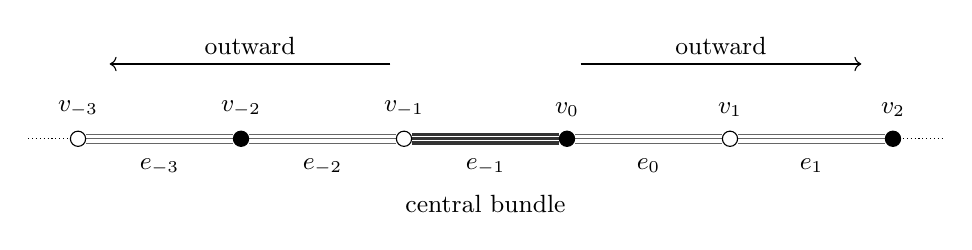
\begin{tikzpicture}[x=1.15cm,y=1cm,font=\small]
  \foreach \a/\b in {-4.5/-2.7,-2.7/-0.9,0.9/2.7,2.7/4.5}{
    \foreach \h in {-0.055,0,0.055}{
      \draw[black!60] (\a+0.09,\h)--(\b-0.09,\h);
    }
  }
  \foreach \h in {-0.055,0,0.055}{
    \draw[very thick,black!80] (-0.81,\h)--(0.81,\h);
  }
  \draw[densely dotted] (-5.05,0)--(-4.61,0);
  \draw[densely dotted] (4.61,0)--(5.05,0);
  \foreach \x/\n in {-4.5/-3,-0.9/-1,2.7/1}{
    \node[circle,draw,fill=white,inner sep=0pt,minimum size=5.5pt]
      at (\x,0) {};
    \node[above] at (\x,0.16) {$v_{\n}$};
  }
  \foreach \x/\n in {-2.7/-2,0.9/0,4.5/2}{
    \node[circle,draw,fill=black,inner sep=0pt,minimum size=5.5pt]
      at (\x,0) {};
    \node[above] at (\x,0.16) {$v_{\n}$};
  }
  \foreach \x/\n in {-3.6/-3,-1.8/-2,0/-1,1.8/0,3.6/1}{
    \node[below] at (\x,-0.13) {$e_{\n}$};
  }
  \draw[->] (-1.05,0.95)--(-4.15,0.95)
    node[midway,above] {outward};
  \draw[->] (1.05,0.95)--(4.15,0.95)
    node[midway,above] {outward};
  \node[below] at (0,-0.59) {central bundle};
\end{tikzpicture}

\caption{Each segment represents a copy of $D$. A copy of $Q$ uses
the two bundles incident with its vertex. Filled vertices contribute
to $M_0$, open vertices to $M_1$. The central bundle is $e_{-1}$;
from either endpoint, the $L$-coordinate points toward the center and
the $R$-coordinate points outward.}
\label{fig:double-ray}
\end{figure}

Every finite subset of $E$ is independent in each $M_i$, because
all its component parts are finite and every finite subset of $Q$ is
independent by Remark~\ref{rem:uniform-local}. But $E$ is dependent
in each $M_i$: its intersection with any component support is the
dependent whole ground set of that copy of $Q$. Thus neither $M_i$
is finitary. Since $M_i=M_i^*$, neither is cofinitary either.

In fact, neither matroid has a nonempty finitary or cofinitary direct
summand. Suppose a nonempty set $F$ supports a finitary summand.
Every subset of $F$ is independent, since all its finite subsets are
independent, so $F$ is the summand's only basis. Thus every basis of
$M_i$ contains $F$. But complements of bases are also bases of $M_i$,
a contradiction. Dualizing the direct-sum basis description gives the
same contradiction for a cofinitary summand.

\subsection{The descending ranks}

Suppose that independent sets $J_i$ of $M_i$ cover $E$.
Replacing $J_1$ by $E\setminus J_0\subseteq J_1$, we obtain an
independent partition $E=J_0\mathbin{\dot\cup}J_1$.
Assign each element of a bundle to the endpoint whose parity agrees
with its part in this partition. At every vertex, the assigned elements
on its two incident bundles form an independent set of its copy of $Q$.

The central bundle is partitioned between $v_{-1}$ and $v_0$.
Exactly one of the two label sets belongs to $\mathcal U$.
Start at that endpoint and move outward forever. Write $x_k\subseteq D$
for the labels received by the $k$th vertex on its inward bundle.
Thus $x_0\in\mathcal U$. If the current vertex receives $z_k$
on its outward bundle, the next vertex receives exactly
\[
 x_{k+1}=D\setminus z_k
\]
there, because the assignment is a partition and the label maps agree.

Assume inductively that $x_k\in\mathcal U$. The independent
assignment at this vertex is contained in a basis $B_k$ of its copy
of $Q$. Put
\[
 u_k=(B_k)_L,
 \qquad y_k=D\setminus(B_k)_R.
\]
We have $x_k\subseteq u_k$, so $u_k\in\mathcal U$.
Equation~\eqref{eq:outward-rank} gives $y_k\in\mathcal U$ and
$\rho(u_k)>\rho(y_k)$. Since $z_k\subseteq(B_k)_R$,
we have $y_k\subseteq x_{k+1}$; hence $x_{k+1}\in\mathcal U$.
Antitonicity now yields
\begin{equation}\label{eq:ordinal-descent}
 \rho(x_k)\ \ge\ \rho(u_k)\ >\ \rho(y_k)\ \ge\
 \rho(x_{k+1}).
\end{equation}
This produces an infinite strictly descending sequence of ordinals,
which is impossible: its set of values has a least element, and the
next value would be smaller.

Thus $M_0,M_1$ have no independent covering of $E$.
By Lemma~\ref{lem:selfdual-reduction}, they have no packing/covering
partition either. Their common ground set is countably infinite and
both matroids are self-dual on the same labels, completing the proof
of Theorem~\ref{thm:main}.

\section{The separate Covering and Packing conjectures}
\label{sec:separate-consequences}

Bowler and Carmesin also formulated separate Covering and Packing
conjectures. For a set-indexed family $\mathcal M=(M_i:i\in\Theta)$ on $E$,
write $\mathcal M\!\upharpoonright Y=(M_i\!\upharpoonright Y:i\in\Theta)$
and $\mathcal M.Y=(M_i.Y:i\in\Theta)$. Their Covering Conjecture asserts,
for every such family, the equivalence
\begin{equation}\label{eq:covering-conjecture}
\begin{aligned}
 &\mathcal M\text{ has a covering}\\
 &\quad\Longleftrightarrow\quad
 \text{for every }Y\subseteq E,\\
 &\qquad\bigl[\mathcal M\!\upharpoonright Y\text{ has a packing}
 \Longrightarrow
 \mathcal M\!\upharpoonright Y\text{ has a covering}\bigr].
\end{aligned}
\end{equation}
Their Packing Conjecture asserts, again for every such family,
\begin{equation}\label{eq:packing-conjecture}
\begin{aligned}
 &\mathcal M\text{ has a packing}\\
 &\quad\Longleftrightarrow\quad
 \text{for every }Y\subseteq E,\\
 &\qquad\bigl[\mathcal M.Y\text{ has a covering}
 \Longrightarrow
 \mathcal M.Y\text{ has a packing}\bigr].
\end{aligned}
\end{equation}
These are the conjectures of~\cite[Conjectures~5.2 and~6.3]{BowlerCarmesin2015}.

\begin{corollary}\label{cor:separate-covering-packing}
The unrestricted separate Covering and Packing Conjectures of Bowler and
Carmesin are both false in ZFC.
\end{corollary}

\begin{proof}
Bowler and Carmesin's universal equivalences identify intersection for
every pair, packing/covering for every pair, packing/covering for every
set-indexed family, \eqref{eq:covering-conjecture} for every set-indexed
family, and \eqref{eq:packing-conjecture} for every set-indexed family
\cite[Section~7]{BowlerCarmesin2015}. Theorem~\ref{thm:main} falsifies the
pairwise packing/covering assertion, so both separate universal conjectures
are false. These last two failures are consequences of equivalence between
universal statements; this argument does not identify their witnessing
families with the pair $(M_0,M_1)$.
\end{proof}


\begingroup\small
\bibliographystyle{plain}
\bibliography{references}
\endgroup
\end{document}
